\documentclass{CUP-JNL-DCE}


%%%% Packages
\usepackage{latexsym}
\usepackage{graphicx}
\usepackage{multicol,multirow}
\usepackage{amsmath,amssymb,amsfonts}
\usepackage{mathrsfs}
\usepackage{amsthm}
\usepackage{apacite}
\usepackage{rotating}
\usepackage{appendix}
\usepackage[authoryear]{natbib}
%%%%

\articletype{RESEARCH ARTICLE}
\jname{Data-Centric Engineering}
%\artid{20}
\jyear{2020}
%\jvol{4}
%\jissue{1}
%\doi{2190-8567}
%\raggedbottom

\DeclareGraphicsRule{.tif}{eps}{.tif.bb}{`tiff2ps #1}

\begin{document}

\begin{Frontmatter}

\title[The use of location-based data to improve traffic forecasting in cities: a case study on volume-delay curves for London]
{The use of location-based data to improve traffic forecasting in cities: a case study on volume-delay curves for London}

\author*[1]{Bingyu Zhao}\email{bz247@berkeley.edu}
\author[2]{Gerard Casey}\email{gerard.casey@arup.com	}
\author[1]{Kenichi Soga}

\authormark{Gerard Casey \textit{et al.}}

\address*[1]{\orgdiv{Department of Civil and Environmental Engineering}, \orgname{University of California, Berkeley}, \orgaddress{ \country{USA}}}
\address[2]{\orgname{Arup}, \orgaddress{\state{London},  \country{UK}}}

\keywords{Big-data crowd-sourced real-time traffic GPS modelling}

\abstract{In many cities across the world traffic congestion has reached chronic levels. Despite many technological disruptions one of the most fundamental and widely used functions within traffic modelling, the volume delay function, has seen little in the way of change since it was developed in the 1960's. Traditionally macroscopic methods have been employed to relate traffic volume to vehicular journey time. These idealised functions attempt to generalise different aspects of an individual road's characteristics in order to create usable functions that do not require a large range of survey requiring inputs. The general nature of these functions enables their ease of use and gives widespread applicability. However, their ability to give results that consider the individual characteristics of a road (i.e. geometry, the presence of traffic furniture, road quality and the surrounding environment) reduces. This research investigates the use of two different data sources (crowd sourced location informed journey times and automated traffic counters)  for  the established models. The crowd sourced GPS informed journey times offer data that is context specific to a location. Automated traffic counters enable the harvesting of traffic count data over similarly fine temporal resolutions. By combining these two sources for  different road types in London, new context specific volume-delay and speed-saturation functions can be generated. This method shows promise in some locations with the generation of robust functions. In other locations it highlights the need to better understand other influencing factors, such as the presence of on road parking or weather events.}

\begin{policy}[Impact Statement]
Volume delay curves are widely used in traffic analysis. They form a critical part of the traffic assignment step in 4 step modelling. More accurate representations of traffic behaviour under congestion using the data sources illustrated here may permit for a better understanding of real world context specific behaviour.
\end{policy}

\end{Frontmatter}

\section{Crowd sourced journey times and automated traffic counter volume-delay functions for London}\label{v_d_ftns}

When the vehicular demand for a road exceeds the ability to supply, a journey time-delay is incurred as a result of the congestion generated. This relationship of traffic volume to time-delay has historically been simplified to macroscopic principles. The individual interactions of increasing and decreasing vehicle volumes result in changes to the journey time on any given link. As traffic volume and therefore density increase on a fixed length link vehicle speed will reduce in order to safely manage the increased volume. This research investigates the pairing of two data sources; crowd sourced location device informed journey times and traffic count data from the Automated Traffic Counter (ATC) system in the Greater London Area (GLA). This section will begin by reviewing the literature on the methods currently employed. A new method is then proposed which aims to satisfy some of the identified limitations in the current methods by using fine resolution data in the form of automated traffic counters and location device informed journey times on a range of roads within the GLA. 

\subsection{Literature review}

There is a range of macroscopic methods used to relate traffic volume to time-delay.

\subsubsection{Bureau of Public Roads method}

The Bureau of Public Roads (BPR) volume-delay curve was developed in the 1960's and is the most widely used function for relating vehicle volume and journey time. Its simple mathematical form and input requirements are attributed to its widespread use \citep{skabardonis1997improved}. There are many different forms of the BPR function as many different organisations have adapted it with various local empirical and/or hypothetical data \citep{mtoi2014calibration} in an attempt to localise the function.

\vspace{2mm}

The general BPR function is mathematically defined as:

\begin{equation}
	u = \frac{u_{0}}{(1 +  \alpha(x)^\beta ) }
\end{equation}

Where:

\vspace{2mm}
\textit{u} = speed

\vspace{2mm}
$u_{0}$ = free flow speed 

\vspace{2mm}
\textit{x} = saturation (volume/capacity)

\vspace{2mm}
$\alpha$ and $\beta$ = coefficients

\vspace{2mm}

In the case of London, TfL have calibrated the BPR function with exhibited traffic counts and thus defined $\alpha$ and $\beta$ values for the area \citep{tfl_modelling_guidelines}.

\vspace{2mm}
$ \alpha = 1.0 $

\vspace{2mm}
$ \beta = 2.0 $
\vspace{2mm}

Despite the popularity of the BPR function it has many limitations, primarily as it was created by fitting a polynomial equation to uncongested freeway data from the 1950's and thus does not reflect modern operating conditions \citep{skabardonis1997improved}.

\subsubsection{Davidson method}

Davidson (1966) proposed a general purpose travel-time formula in 1966 and this method has undergone numerous modifications since it was first proposed \citep{mtoi2014calibration}. Its popularity is as a result of its flexibility and applicability for a range of contexts (Taylor, 1997). It has exhibited a closer match to actual volume counts and has a stronger theoretical base than the BPR \citep{rose1989estimating}. There have been modifications of the Davidson function since it was first proposed (e.g \citep{tisato1991suggestions}, \citep{akcelik1991travel} ) with the mostly widely used being the Akcçlik functions.

\subsubsection{Akclik method}

The Akclik method is a time-dependent modification of the Davidson model which uses the coordinate transformation technique in an attempt to overcome the conceptual and calibration issues with the Davidson method \citep{akcelik1991travel}. It has illustrated good results in certain road types, tolls roads and signalized arterials \citep{mtoi2014calibration}. 

\subsubsection{Conical method}

Spiess \citep{spiess1990technical} proposed the conical method in 1990. It attempted to overcome some of the upper bound BPR limitations through the use of hyperbolic conical sections whilst maintaining a similar form to the BPR and thus enabled a direct transfer of parameters.

\subsubsection{Identified limitations}

These idealised functions attempt to generalise different aspects of an individual road's characteristics in order to create usable functions that do not require a large range of survey requiring inputs. The general nature of these functions enables their ease of use and gives widespread applicability. However, in doing so their ability to give results that consider the individual characteristics of a road (i.e. geometry, the presence of traffic furniture, road quality and the surrounding land use) reduces. Such differing characteristics can result in very different vehicular behaviour on roads that may be considered similar by these functions. The literature has identified the need to inform these functions with empirical and context specific data \citep{rose1989estimating}, \citep{spiess1990technical} but recognised the difficulty and cost associated with collecting such empirical data as being prohibitive \citep{rose1989estimating}.

\subsubsection{Input data}

There have been studies that incorporate different forms of field sensor data \citep{mtoi2014calibration}, \citep{neuhold2014volume} in volume delay functions. However, the data used in these studies has been generated specifically for that application and requires specific hardware and/or software for use. Recent hardware and software innovations have led to the increased use of real-time crowd-sourced data feeds generally in transport modelling. This includes applications of location data for emissions estimations \citep{hirschmann2010new}, origin and destination matrices \citep{toole2015path} and general urban traffic management applications \citep{artikis2014heterogeneous}. This research investigates the use of new, real-time crowd-sourced data feeds that have a wider spatial spread and are in some cases not generated specifically for this application. These sources may be used to consider some of these previously ignored characteristics and create temporally and spatially dynamic volume, speed and saturation relationships. Such data sources can harvest data at a finer resolution over a longer (even indefinite) period of time giving a far greater understanding of the temporal variations and trends exhibited on road infrastructure.

\subsection{Automated traffic counters}

Automated Traffic Counters (ATCs) are magnetic induction loops located in the road surface. The passing of a vehicle results in an electromagnetic signal. The ATCs in the Greater London Area count every vehicle which passes over the inductions loop. The data used here was harvested over a period from the 29th February to the 21st March 2016.

\subsubsection{Location of ATCs in Greater London}

There are 37 Department for Transport (DfT) ATC locations in the Greater London Area. Most of these locations operate in both directions (34) with others operating only in one direction (3). These ATC locations cover a range of different DfT defined road classes (Table \ref{tab:table3.5}). Guidance on the road classification system in the UK is published by the DfT \citep{DfT_road_classification}.

\begin{table}[h!]
	\centering
	\caption{ATC locations by road class}
	\label{tab:table3.5}
	\begin{tabular}{cc}
		\toprule
		Road Class & Count\\
		\midrule
		Trunk & 6\\
		Principal & 16\\
		B & 3\\
		C & 3\\
		Unclassified & 9\\
		\bottomrule
	\end{tabular}
\end{table}

These ATCs are distributed across the Greater London Area as is shown in Figure \ref{fig:Picture3.22}.

\begin{figure}[htbp!] 
	\centering    
	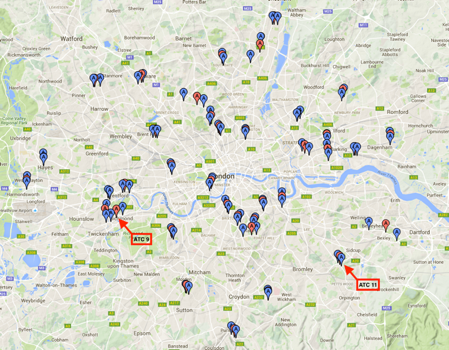
\includegraphics[width=0.75\textwidth]{Picture22}
	\caption[Map of ATC locations in the Greater London Area]{ATC Locations in Greater London Area \citep{google_maps} with DfT data. The red flag illustrates the location of the ATC itself. The blue flags illustrate the origin and destination locations specified in order to harvest journey time information}
	\label{fig:Picture3.22}
\end{figure}

\subsubsection{Raw ATC data}

The raw ATC data contains individual records for each vehicle that passed. Over the test period of 3 weeks there were approximately 4.5million records of vehicles at individual points. For illustration, Table \ref{tab:table3.6} shows a representative sample from the first day of these records at ATC 11 (as labelled in Figure \ref{fig:Picture3.22}). 

\begin{table}[h!]
	\centering
	\caption{Raw ATC data record sample}
	\label{tab:table3.6}
	\begin{tabular}{ccccc}
		\toprule
		Site & Direction & Date & Time & Speed\\
		\midrule
		11 & Northbound & 2016-02-27 & 00:00:28 & 37\\
		11 & Northbound & 2016-02-27 & 00:01:19 & 40\\
		11 & Northbound & 2016-02-27 & 00:02:25 & 42\\
		\bottomrule
	\end{tabular}
\end{table}

\subsubsection{Manipulated ATC data}

In order to combine this data with the temporal journey times, individual vehicle records must be combined hourly in order to find the total volume on that link, per hour. A Python \citep{python_language} script using the Pandas \citep{python_pandas} data library was used for this processing. First, a unique identifier was formed by concatenating the site and directionality of the ATC. The time stamp was rounded up to the next hour in order to quantify the total volume per hour leading up to the journey time taken, up to that hour. This resulted in an output which featured traffic counts per hour (volume) for a site, direction and date, as is sampled and shown in Table \ref{tab:table3.7}.

\begin{table}[h!]
	\centering
	\caption{Processed ATC data record sample}
	\label{tab:table3.7}
	\begin{tabular}{cccccc}
		\toprule
		Site & Direction & Date & Hour & Count & id\\
		\midrule
		9 & Southbound & 2016-02-27 & 13 & 1206 & 9S\\
		9 & Southbound & 2016-02-27 & 14 & 1222& 9S\\
		9 & Southbound & 2016-02-27 & 15 & 1408& 9S\\
		9 & Southbound & 2016-02-27 & 16 & 1604& 9S\\
		\bottomrule
	\end{tabular}
\end{table}

\subsection{Crowd sourced journey times}

\subsubsection{Location data}

Location capable mobile phones have enabled the harvesting of fine resolution temporal and spatial data. The location of a device may be inferred from the use of GPS, cell tower triangulation, WiFi SSID mapping, Bluetooth and other technologies, either in isolation or in tandem. Such data holds a great deal of promise due to the range of possible uses it has in the transportation sector \citep{zheng2010understanding}. The anonymous crowd-sourced collection of this data can be used to derive road traffic conditions \citep{google_traffic_blog}. Such a traffic condition method is well suited to areas of high density, high travel demand and high mobile phone uptake, such as a city. This information is used by many providers who provide real-time traffic informed shortest path directions as a service. For example Apple (\textit{apple.com/ios/maps}), Bing (\textit{bing.com/map}), Google (\textit{google.com/maps}) and TomTom (\textit{tomtom.com}). These services are generally used by individuals who wish to make an informed decision on route choice for a given mode or even a mode decision on how to get from their starting point to a desired destination. The aim of this research was not to make use of the shortest path algorithm or large-scale computational power of these service providers, but to access a more localised, location device informed, journey time on a fixed and relatively short stretch of road. 

\subsubsection{Google Maps}

This research makes uses of Google's traffic information through the Google Maps Directions \citep{Google_directions_api} Application Protocol Interface (API). Dependent on their personal settings, an Android user or other Operating System (OS) user, with the free Google Maps mobile app installed on their location enabled phone send anonymous data to Google. Such data is personally and commercially sensitive and so post-processing is carried out by Google in order to ensure that no-one user's movements can be isolated from the flows.  

Google's traffic maps can be visually inspected through their maps interface on any modern web browser on google.co.uk/maps. Their colour coded scale gives a qualitative feel for traffic conditions on the roads where Google have sufficient data, as is shown in Figure \ref{fig:Picture3.23}. Such qualitative data is only useful for contrasting different traffic states on a road. 

\begin{figure}[htbp!] 
	\centering    
	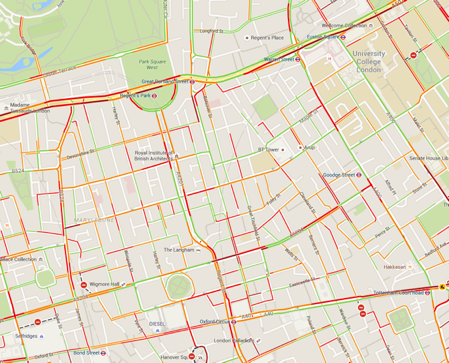
\includegraphics[width=0.75\textwidth]{Picture23}
	\caption[Google Maps Traffic Layer, Camden/Soho/Marylebone/Mayfair area of London  \citep{google_maps}]{Google Maps Traffic Layer, Camden/Soho/Marylebone/Mayfair area of London  \citep{google_maps}}
	\label{fig:Picture3.23}
\end{figure}

\subsubsection{Google Maps Directions API}

The Directions API is a service that calculates directions between locations using a Hypertext Transfer  Protocol (HTTP) request \citep{Google_directions_api}. The use of a HTTP request allows for scheduled and bulk harvesting of journey information between given origin and destination pairs. The aim of this research was to combine crowd-sourced location device informed journey times with traffic counts from the DfT ATC network. As such, the first step was to specify origins and destinations for the Google Directions HTTP request that would provide a journey time for the traffic counts at defined ATC locations. There is a need to convert from EPSG:27700 (British National Grid), as provided by the DfT for ATC locations, to the EPSG:4326 (WGS84) as used by Google Maps. The ATCs take a point measurement at a defined location along the road link. In order to find a journey time along that road, an origin and destination location definition process is required. In deciding on origin and destination pairs a balance must be made between having sufficient distance in order to get meaningful journey time results and having sufficiently short distance so as to not include other phenomena such as junctions and intersections. Consider ATC location 6 Eastbound, the A205 Dulwich Common SE21 in the Borough of Southwark. In Figure \ref{fig:Picture3.24} the location and defined origin and destination points can be inspected. Automating the definition of these origin and destination pairs was challenging as simply taking the start/end of a given road often gave a route that was too long and thus was distorted by other traffic, outside of the ATC consideration. Other methods based upon an idealised distance between points and the density of junctions was deemed too complex and not durable. For bidirectional ATC locations it was often not possible to define the Eastbound route as the inverse of the Westbound route as Google distinguish between different sides of the road, resulting in a route which involves a detour to safely navigate to the correct orientation.  Thus a manual process was employed to visually inspect each location, the surrounding context and decide on the most appropriate O/D pair. Once this manual process was complete, a matrix of origin and destination pairs was produced containing ATC metadata that will allow for the pairing of Google results to its corresponding ATC data. 

\begin{figure}[htbp!] 
	\centering    
	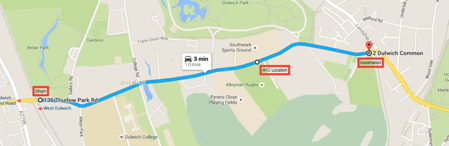
\includegraphics[width=0.65\textwidth]{Picture24}
	\caption[ATC 6 Eastbound with defined origin and destination points \citep{google_maps}]{ATC 6 Eastbound with defined origin and destination points \citep{google_maps}}
	\label{fig:Picture3.24}
\end{figure}

\subsubsection{Sending HTTP request to Google}

A HTTP request is made in Python to Google's servers with the origin, destination, mode (driving) and the specified departure time. In order to harvest real-time data that is informed by location device information at that time the departure time is set to the live time and a scheduler is used to run the same origin and destination pairs repeatedly. Cron, a time-based scheduler for Unix operating systems, was used to run the Python HTTP request every hour for the given dates of the study. 

\subsubsection{Receiving JSON response from Google}

In response to the HTTP request Google returns results in JavaScript Object Notation (JSON, see \textit{json.org}), a lightweight data-interchange format. At the time of writing the JSON response contains 3 root elements, the status, geo\_coded waypoints and the routes. Within routes the key metric of duration\_in\_traffic for the requested route is found, stating the estimated journey time on the route, at that time. The entire JSON response is parsed and transferred to a MySQL (\textit{mysql.com}) relational database for temporary storage. From the database, the origin, destination, ATC related data and the key duration\_in\_traffic metric can be paired with the ATC counts.

\subsubsection{Data cleaning}

Prior to combining the two data sources the Google data was sense checked. A small number of Google results returned no duration\_in\_traffic field. These results were likely due to low density of location device data as a result of low user demand or poor location device signal reception in that location. This included three ATC pairs (ATC numbers 42, 48 and 74 in both road directions) and one ATC (36N) in one direction. They were discarded so as not to skew the results. It was also noted that at times of low demand (late night and early morning) the duration\_in\_traffic response did not return and it can therefore be deduced that duration\_in\_traffic was only returned when there is sufficient spatial and temporal resolution location device input data. 

\subsubsection{Data validation}

Google's methodology nor location device sample information is available for commercial and privacy reasons. Since there are no comparable, freely available data sources, the Google API responses pose a validation challenge. It is therefore an assumption that these responses present location device informed journey times.

\subsection{Analysis}

The combination of Google data and DfT ATC vehicle count data enables various relationships to be assessed and defined. In this section a number of these relationships are discussed. For the purposes of comparison, the widely used BPR functions are shown in tandem.

\begin{figure}[htbp!] 
	\centering    
	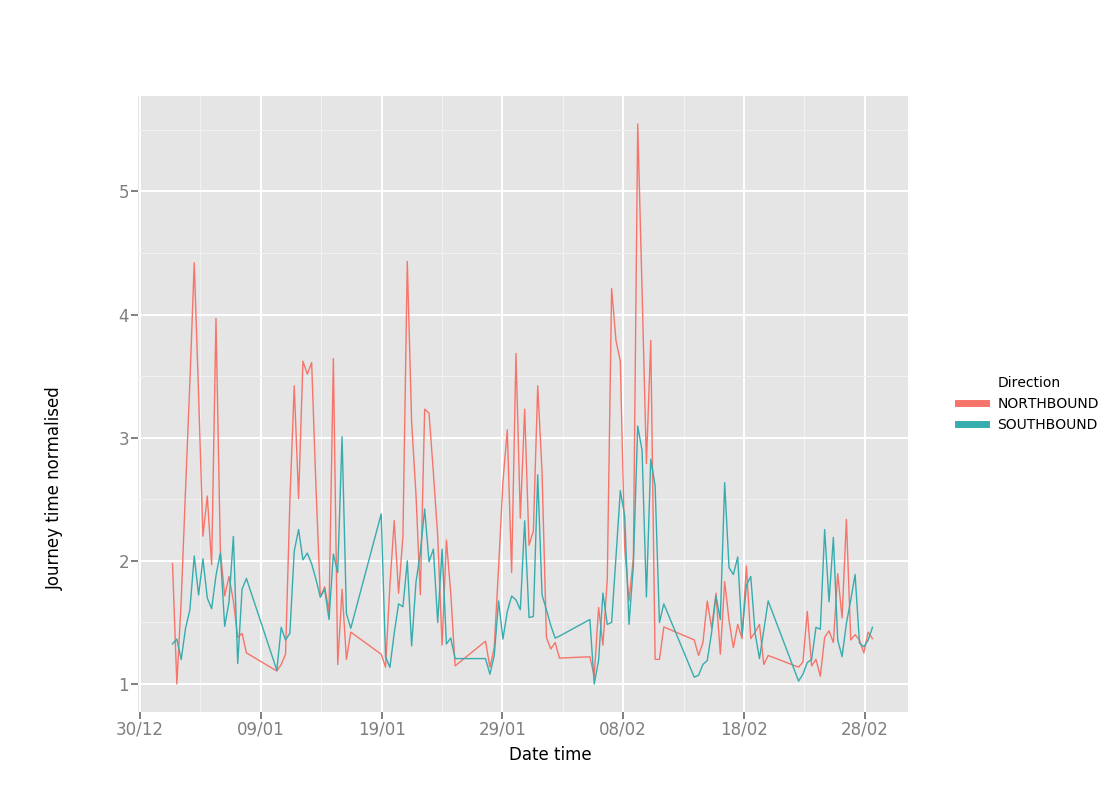
\includegraphics[width=1.0\textwidth]{Picture25}
	\caption[Journey time distribution Location 67 (7th-13th March 2016)]{Journey time distribution Location 67 (7th-13th March 2016)}
	\label{fig:Picture3.25}
\end{figure}

\subsubsection{Journey time distribution}

The Google data was analysed to assess the vehicle traffic distribution pattern. Vehicle traffic distribution is generally modelled as a daily bimodal distribution with peaks associated with the morning (to work) and evening (leaving work) periods \citep{mullick2012dynamics}. It is generally expected that the load will lean on the city inbound direction in the morning and then on the city outbound direction in the evening. Figure \ref{fig:Picture3.25} displays a one-week sample of ATC location 67 in both the northbound and southbound directions. Location 67 is situated on Buckingham Palace Road, A3214 with the northbound direction leading to central London and the southbound direction heading away from central London. In order to make journey time comparisons, the journey time delay is normalised. 

The normalised time delay is defined as:

\begin{equation}
	time delay_{norm} = \frac{Journey time}{Journey time_{0}}
\end{equation}

\vspace{2mm}

Journey $time_{0}$ is taken as the minimum exhibited journey time on the road link. Journey $time_{0}$ is also referred to as the free flow journey time and is usually found in the early hours of the morning. This empirical method deviates from the standard method of defining the free flow journey time which generally relies on using time delay coefficients for different road types, speed limits, link lengths, widths, gradients, traffic junctions and so on \citep{DfT_cost_benefit}.

In this study, it is recognised that such an assumption negates the impact of context specific information such as road geometry or road furniture. Rather than making assumptions about the free flow journey time it was taken as being the lowest exhibited time from the Google journey time data over the period of the study.

In Figure \ref{fig:Picture3.25} the x-axis displays normalised journey times as a ratio of the free flow journey time (t/$t_{0}$) and the y-axis displays these journey times over seven days at one-hour resolution. On first inspection, the seven different days are clear. The late night and early morning periods display the lowest journey times, approaching $time_{0}$. The northbound direction, towards the city centre, exhibits the largest load in the mornings and interestingly, peaks on a Friday evening. The southbound, away from the city centre direction peaks daily in the afternoon and similarly to the northbound lane, has its weekly peak on a Friday evening. Saturday and Sunday show distinct behaviour to weekdays, with overall reduced journey times in both directions and a proportionally higher journey time on the southbound, away from city lane, in contrast to weekday behaviour.  It is clear from this alone that even the categorisation of journey times as weekend vs weekday distributions \citep{mullick2012dynamics} is problematic, as each day exhibits its own distinct behaviour.

\subsubsection{Saturation-delay relationship} \label{sat-delay}

By combining the Google journey time data with the ATC vehicle count data, volume delay curves may be plotted. In order to facilitate comparisons, the vehicle volume is converted to saturation where saturation is defined as:

\begin{equation}
	saturation = \frac{volume}{capacity}
\end{equation}

Defining capacity is challenging as there are a range of possible definitions:

\begin{enumerate}
	\item Free flow capacity - the maximum vehicle volume before a time-delay is incurred
	\item Maximum flow capacity – absolute vehicular volume a road can carry with no regard to time-delay
	\item The UK Design Manual for Roads and Bridges (DMRB) qualitative capacity definition - “capacity is defined as the maximum sustainable flow of traffic passing in 1 hour, under favourable road and traffic conditions.” \citep{DMRB}
\end{enumerate}

The DMRB provides look up tables that feature traffic capacities for a range of road types, road widths and number of lanes. A manual survey of satellite imagery was carried out to assess the lane count, estimate the road width for each of the ATC locations and thus provide an estimated capacity by this DMRB definition. However, such a method was deemed unacceptable due to the uncertainty in what constitutes ‘\textit{favourable road and traffic conditions}.’

Instead, a more nuanced definition was adopted from Spiess \citep{spiess1990technical} which defined capacity as the volume at which congested speed is half the free flow speed. The paired Google and ATC data was queried to find the estimated volume when the vehicle's speed was 50\% of the free flow (minimum) journey time ($time_{0}$). As a result, individual roads are given a capacity attribution. This capacity attribution is generally lower than that from those which are more qualitative. 

Consider Figure \ref{fig:Picture3.26} which illustrates the saturation-delay curve for ATC locations 19E, 35S, 19 (both) and 15 (both). The top left figure presents the raw saturation time delay data with two curves, the BPR function and a third order polynomial regression function ($Adj. R^2$=0.73) for the given data. The function derived from the empirical data closely matches the BPR function with some small deviances at very low and very high saturation ratios. In this example, the road experiences a healthy amount of demand and this is reflected in a maximum saturation of less than 120\%. 

Other locations experience much higher peak loads, resulting in a different functional relationship. Figure \ref{fig:Picture3.26} top right presents the saturation time delay curve for ATC location 35S. This road experiences higher demands than ATC 19E and exhibits saturation levels approaching 150\%. In this case, the BPR function deviates significantly from the empirical data from 50\% saturation and approaches a 2-fold time difference as it approaches a saturation level of 150\%. For this particular location the empirical data suggests that an increase in volume does not have as significant effect on journey times as the BPR function would model.

Different direction road lanes share similar geometry with individual characteristics and experience different demands at different times. A comparison can be made of their individual saturation delay curves in order to assess their individual characteristics. Figure \ref{fig:Picture3.26} bottom left illustrates location 19 in the eastbound and westbound directions. The two directions exhibit distinct behaviour despite being the same road. The westbound direction exhibits large time delays at high saturation levels, peaking at a 5-fold increase over free flow journey time.  The eastbound direction does not have such a time delay peak. As a result, their individual regression lines differ, with a steeper curve westbound and a gradual curve eastbound. The BPR function falls between these functions and reflects what is close to an average condition when collectively considering both directions. 

Figure \ref{fig:Picture3.29} bottom right displays ATC location 15 where again distinct directionally dependent behaviour is exhibited. The Northbound direction exhibits a higher capacity to absorb traffic volume, showing a lower rate of time delay increase for a substantially larger increase in saturation. Saturation levels peak at nearly 2 illustrating that the use of the Spiess \citep{spiess1990technical} methodology for capacity definition has a significant impact on saturation. Such a metric would generally not be exhibited using the kind of qualitative definitions discussed previously. There is a contrasting relationship to the BPR function. It is shown to highly overestimate the time delay from the point of 50\% saturation. It is clear that both lanes exhibit a greater capacity to accommodate increased vehicle demand with a reasonable time-delay than the BPR functions predicts.

\begin{figure}[htbp!] 
	\centering    
	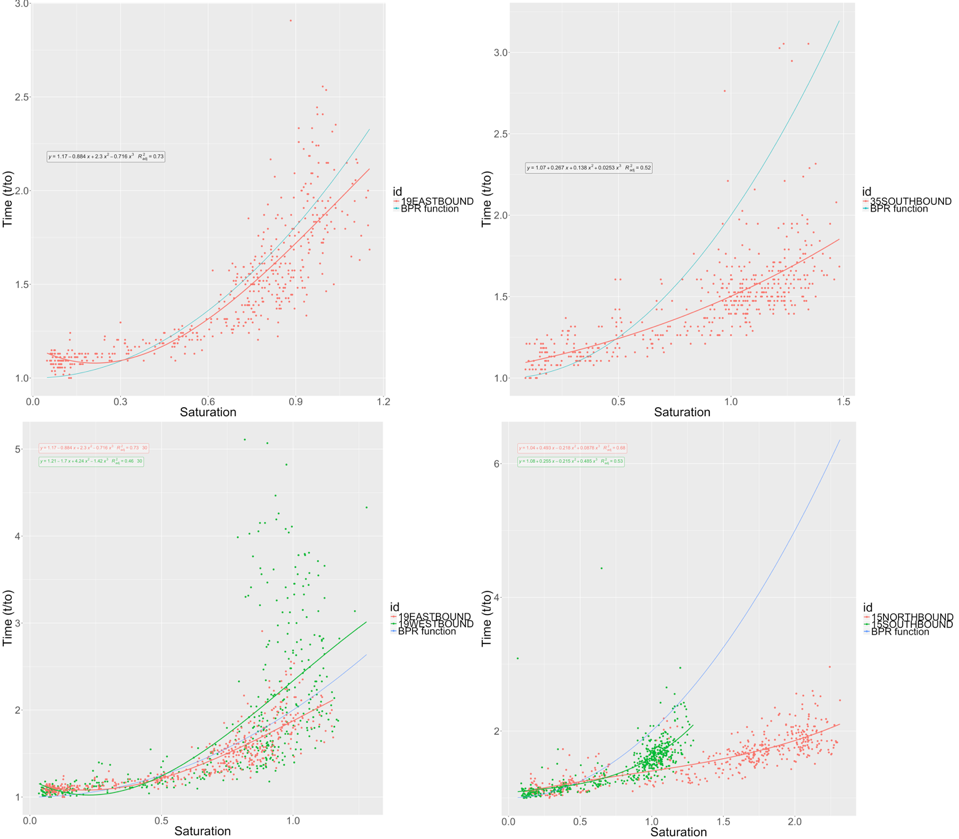
\includegraphics[width=1.0\textwidth]{Picture26}
	\caption[Saturation time delay curve ATC 19 Eastbound (top left), 35 Soutbound (top right), 19 (bottom left),15 (bottom right)]{Saturation time delay curve ATC 19 Eastbound (top left), 35 Soutbound (top right), 19 (bottom left),15 (bottom right)}
	\label{fig:Picture3.26}
\end{figure}

\vspace{5mm}
\textit{Upper \& lower bounds}
\vspace{5mm}

Volume delay functions have significant issues at their lower and upper bounds. At the lower bound, there is the challenge of distinguishing between vehicular volume up to the point of free flow and at the upper bound limiting vehicular volume by the maximum flow capacity. 
In the lower bound a probabilistic method can be employed to handle the uncertainty in vehicle volumes. The raw DfT ATC traffic counts provide vehicular volume distributions 24 hours per day and as such those points which fall in the lower bound, generally late night and early morning can be used to define a volume distribution. Thus, in the situation where a volume delay function is employed to estimate the traffic volume for a time-delay ratio of 1, an estimated traffic volume can be given dependent on the time of day of the query.

The upper bound poses a different challenge. The peak exhibited journey times (defined here as > 3 times free flow journey time) are usually attributable to external factors and not simply vehicle to vehicle interactions. Examples of the external factors include road traffic accidents, weather events or road maintenance. In such situations it is possible for journey times to reach many times the free flow journey time. For illustration, ATC 11N had a journey time 6.85 times greater than the free flow journey time on the 1st March at 9am. A cached internet search highlighted emergency road works at this location due to a burst water main (\textit{http://bit.ly/1ZYxzQ0}). In such a case the estimated vehicle volumes are greatly overestimated by the volume delay function and there is therefore a need to present a constraining factor, maximum flow capacity. 

\begin{table}[h!]
	\centering
	\caption{Upper \& lower bound distribution of volume delay ratio analysis}
	\label{tab:table3.8}
	\begin{tabular}{ccc}
		\toprule
		Bound & Definition & Percentage \\
		\midrule
		Lower & < 1.1 time ratio & 7.56\% \\
		Upper & > 3.0 time ratio & 1.14\% \\
		\bottomrule
	\end{tabular}
\end{table}

In order to assess the frequency of this challenge the data was analysed to better understand the frequency of the lower and upper bound conditions. The results are presented in Table \ref{tab:table3.8}. For the lower bound a conservative estimation was taken with the frequency of time ratio less than or equal to 1.1 in order to capture possible driving style fluctuations above the free flow journey time. These values constituted about 7\% of the total sample. The upper bound, defined as greater than or equal to 3 times free flow journey time was about 1\% of the sample. This illustrating that the lower bound conditions are relatively rare in a high density, high demand area such as London and that this condition is only ever met at periods of little concern, late night and early morning. The upper bound conditions were even more rare, at 1\% of the sample.

In conclusion, the lower bound problem constitutes an issue at times of little concern and very low demand, late night and early morning. A probabilistic solution can be used to interpolate and provide estimated values if needed. On the other hand, the upper bound problem is a much less prevalent than the lower bound problem but is much more profound in that it has a huge impact on travellers and generally hits at high impact ‘rush hour’ times. A constraining factor is required to contain the volume delay function in such a case. Another feature of upper bound conditions is that they involve a large number of travellers (in contrast to lower bound conditions) and as such their impact is more significant. The incidents that lead to the upper bound issue are discussed in terms of possible data sources and predictive inclusion illustrated previously.

\subsubsection{Saturation-speed relationship}

The vehicle speed can be plotted against the saturation ratio in order to relate the impact of vehicle volume on the resulting vehicle speed. The saturation-speed relationship for ATC location 19E is illustrated on the left in Figure \ref{fig:Picture3.27}. A third order polynomial fit is given for each direction ($Adj. R^2$ Eastbound = 0.84, $Adj. R^2$ Westbound = 0.74) of the data is presented in contrast to the BPR function. The empirical data shows a significant overestimation by the BPR function at low values of saturation, showing that average speeds do not approach the given speed limit on this road. The function's converge at a saturation level of 60\% to the Eastbound lane and match relatively closely at higher levels of saturation. Again, it is clear that the roads have unique behaviour dependent on directionality. They share the same shape but the westbound lane exhibits speeds 4 \textit{m/s} slower than the eastbound lane at the same saturation ratio. It also shown again that the BPR function over overestimates speeds at low saturation, reinforcing the conclusion that drivers often don't approach the road's maximum permissible speed even when it may be legally possible to do so. Figure \ref{fig:Picture3.27} on the right presents a speed saturation curve where the BPR curve illustrates a different shape to that of the empirical data. Again, it overestimates vehicle speeds at low saturation levels and predicts a larger range of speeds than those exhibited. The differences between the north and southbound lanes is again present, although not to the same degree as ATC 19. A relatively constant 1.25 \textit{m/s} speed difference is found between the two-lane directions for the same saturation level.  The BPR function is highly dependent on the free flow journey time which has been defined as a function of link speed and length. The shape of the BPR function reasonably matches the empirical data in these cases but often presents locational errors in those sites were the speed limit is rarely, if ever met by drivers in real-world conditions.

\begin{figure}[htbp!] 
	\centering    
	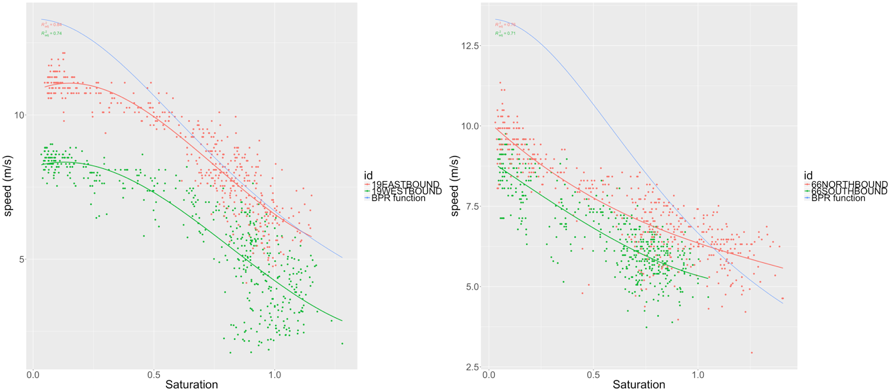
\includegraphics[width=1.0\textwidth]{Picture27}
	\caption[Speed saturation curve ATC 19 (left) and 66 (right)]{Speed saturation curve ATC 19 (left) and 66 (right)}
	\label{fig:Picture3.27}
\end{figure}

\subsection{Discussion}

In many cases, the plots generated in this study presented empirical data that did not match the conventional macroscopic understanding, as epitomised by the BPR functions. For each direction and each individual site, a third order polynomial fit was generated to create context specific saturation delay and saturation speed functions. The $Adj. R^2$ for these generated functions has been plotted as a probability frequency distribution function (density) plot in Figure \ref{fig:Picture3.28} in order to assess the confidence of the derived functions. Interestingly the saturation speed functions exhibited greater predictive ability than the saturation delay functions. The speed metric is derived from the time-delay metric by considering the fixed length of the road, thus the two functions share a similar shape. It is clear that some derived functions have low confidence and there are external unknown factors that have not been considered. 

\subsubsection{Example scenario \& possible factors} \label{factors}

Figure \ref{fig:Picture3.27} presented a speed saturation plot for ATC66 in both directions. In an attempt to better understand and possibly explain this distinct directional behaviour, satellite photography and street level photography of the road was assessed. Figure \ref{fig:Picture3.29} shows a satellite image of ATC66. The red marker gives the location of the ATC counter itself and the two blue markers illustrate the origin/destination location (dependent on direction) for the Google Directions API request. The speed saturation plot (Figure \ref{fig:Picture3.27}) shows a significant speed reduction for traffic in the southbound direction to that of traffic in the northbound direction. From the satellite imagery and street view imagery \citep{Google_street_view} possibly explanatory factors can be identified:

\begin{enumerate}
	\item The southbound lane features on road parking
	\item The southbound lane features a large bus stop and taxi lay-by (for Leytonstone Station) and a smaller bus stop lay-by
\end{enumerate}

The larger bus stop and taxi lay-by serving Leytonstone is a significant geometric feature that is likely to have heavy impacts southbound traffic as buses/taxis leave and enter from both directions on the road. The second smaller bus stop lay-by and on-road parking may also have an impact, albeit in a smaller way to the traffic speed in the southbound direction. Such factors may explain the exhibited differences from the location device informed journey data and thus permit their inclusion in an informal way.

\subsubsection{Challenging scenarios}

A subset of roads presented results that did not resemble previously defined functions. Consider Figure \ref{fig:Picture3.30} which presents the saturation time delay curves for ATC location 9 in both directions on the left. Visually it can be seen in the lower part of the plot that there are the same general trends discussed in Section \ref{sat-delay} but with a large amount of highly variable journey time outliers. There are over 20 points that exhibit journey times over twice the length of the minimum exhibited journey time, peaking at 7 fold increases. These outliers result in low correlations for a second order polynomial fit ($Adj. R^2$ of 0.071 southbound and 0.16 northbound). Such extreme differences may be explained by events such as weather or road traffic incidents, for example a road traffic collision or road flooding as a result of high level of precipitation in a short period of time. Figure \ref{fig:Picture3.30} presents the saturation time delay curve for ATC 67 in both directions on the right. A chaotic pattern of saturation time-delay data is given and little order is evident. Two second order polynomial fits are presented and as is visually evident offer little in the way of a robust function, presenting an $Adj. R^2$ of 0.05 northbound and $Adj. R^2$ of 0.22 southbound respectively. 

\begin{figure}[htbp!] 
	\centering    
	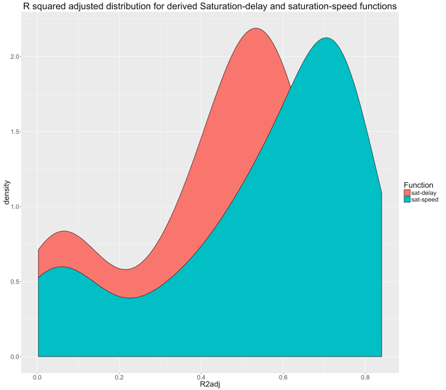
\includegraphics[width=0.7\textwidth]{Picture28}
	\caption[$R_{2Adj}$ probability density function for derived saturation-delay and saturation-speed functions]{$R_{2Adj}$ probability density function for derived saturation-delay and saturation-speed functions}
	\label{fig:Picture3.28}
\end{figure}

\begin{figure}[htbp!] 
	\centering    
	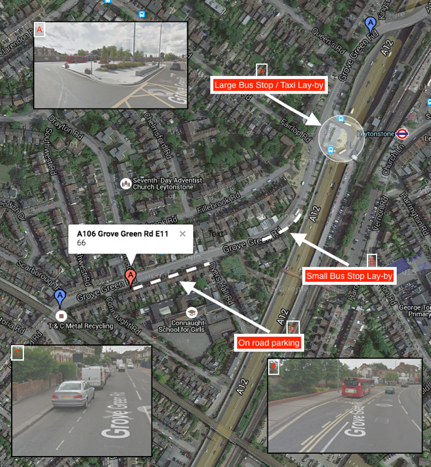
\includegraphics[width=0.7\textwidth]{Picture29}
	\caption[Satellite \& Street View images of ATC 66 \citep{google_maps}]{Satellite \& Street View images of ATC 66 \citep{google_maps}}
	\label{fig:Picture3.29}
\end{figure}

\begin{figure}[htbp!] 
	\centering    
	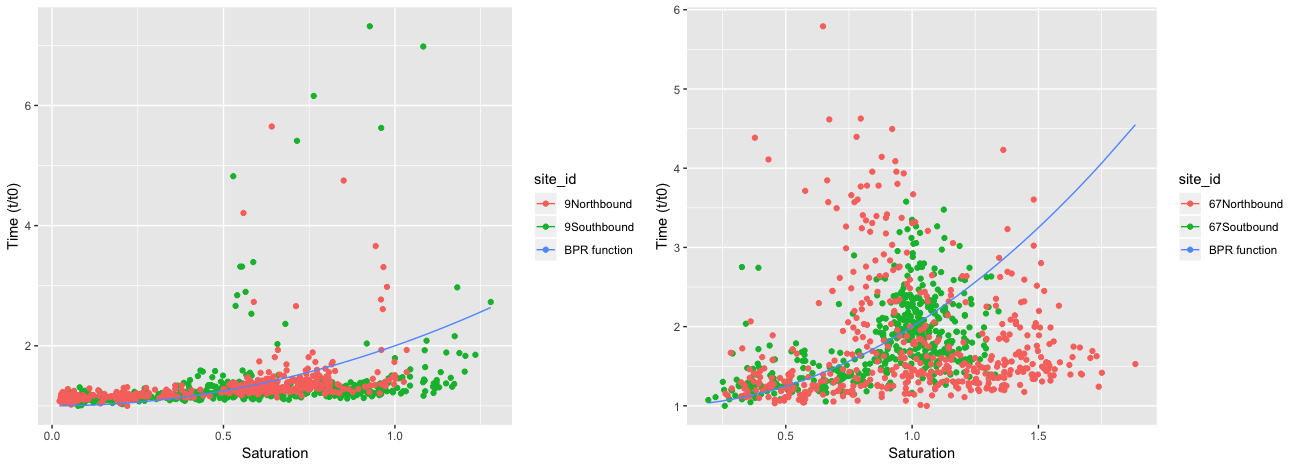
\includegraphics[width=1.0\textwidth]{Picture30}
	\caption[Saturation time delay curve ATC 9 (left) and 67 (right)]{Saturation time delay curve ATC 9 (left) and 67 (right)}
	\label{fig:Picture3.30}
\end{figure}

\subsubsection{Influencing factors}\label{other_factors}

It is clear from these plots that there are factors not considered in this analysis that may help explain the unexplained variations. In Section \ref{factors} the existence of public transport infrastructure and on-road parking were identified as being potentially explanations of the distinct southbound northbound behaviour on that road. A range of possible factors have been identified:

\begin{enumerate}
	
	\item Vehicle type
	
	Further work is planned to assess the impact of the vehicle type. In this paper each vehicle has been attributed equally despite the clear distinction between the interactions of a car and another car compared to that of a lorry to a car \citep{vap2007investigating}. A wide variety of vehicles mixes are exhibited on different road types and such differences should be considered. The use of statistical vehicle mix sampled by road type \citep{DfT_car_stats} was discounted for this study due to the small sample size of such statistics compared to the resolution of the data used here. The use of traffic cameras with number plate recognition and sufficient privileges to the Driver and Vehicle Licensing Agency database would enable the disaggregation of vehicle type at a similar spatial and temporal resolution to the Google Directions and DfT ATC data presented here. 
	
	\item Weather
	
	Weather events may impact on journey times by impacting on the performance of the vehicle, the performance of the road and/or the performance of the driver. Ongoing research at the University of Cambridge is combining a large dataset of Google Directions journey times with data from the UK's Met Office NIMROD precipitation dataset \citep{met_office} in order to assess the relationship between these variables. At the microscopic level it is known that an increase in precipitation increases journey times as a result of increased risk and the resulting decrease in vehicle speeds to compensate for this \citep{mashros2014impact}. 
	
	\item Road incidents 
	
	Road works and road traffic collisions can lead to decreased or even zero capacity on a road link, resulting in increased saturation and thus impacting on journey time. Depending on the warning before such an event, the vehicle traffic may have the ability to adjust to this information, resulting in a greater distribution of traffic, leading to mediated travel times. Alternatively, an accident may occur and not enable any warning to be given to other road users until they are committed to their route choice, resulting in large journey time increases, perhaps explaining extreme phenomena. A method incorporating different accident and road works databases with Google Directions data is currently being investigated.
	
	\item Road geometry, type \& land use
	
	Different road layouts may result in an increase in the complexity of vehicle interactions. For example, the curvature of a corner and the road surface quality will impact on the speed of a vehicle. The surrounding land use will likely also impact, adding safety concerns (for example a school or leisure centre) again impacting on vehicle speed. The inclusion of such factors poses many challenges, the size and complexity of the data plus the uncertainty and variability in how drivers react to the data.
	
	In Figure \ref{fig:Picture3.29} a series of geometric factors are displayed as part of an attempt to explain different behaviour on the same road dependent on direction. The factors discussed there, on-road parking and bus lay-bys may be quantitatively captured using machine vision and data sources such as Google Street View.
	
\end{enumerate}

\subsection{Conclusions}

A range of context specific saturation time-delay, speed saturation and journey time distribution curves for a range of different locations and road types have been generated. Specific examples have been presented here for discussion and all generated functions and plots are available for inspection here. In the most practical sense some of these functions may now be used in the traffic assignment stage of the traditional four step model. In some cases, the data presents clear evidence that unknown factors, such as those listed in Section \ref{other_factors}, have a significant impact and warrant further investigation. In these cases the derived functions and indeed any standardised function have been shown to deviate significantly from empirical data and as such their use should be considered with care. This said, the probability frequency distribution in Figure \ref{fig:Picture3.28} describes the significant collective correlations between the ATC traffic count data and that of the Google journey times, across a range of sites, presenting evidence which goes some way to validate the Google data and illustrate the collective value of this method. The data used here shows promise in considering the tangible factors which impact on road performance, such as local geometry, bus stops and so on, but that have historically been too challenging to be considered. These data sources have longevity, exist at close to real-time and in the case of the Google Directions data, relatively low cost with little or no capital expenditure required for its harvesting. These methods may be employed over a long time horizon and at a finer temporal resolution in order to better understand the temporal and spatial trends as well as the influencing factors such as sporting occasions and weather events. It can also be used to do real-time vehicle emissions estimations and modelling, as is being investigated presently. The automation of this method over longer time horizons may lead to explanations for the issues discussed previously and highlight areas that require investigation in order to better understand the performance of road infrastructure.

\begin{Backmatter}

\paragraph{Acknowledgments}
We are grateful to both Google and the Department for Transport for access to data. 

\paragraph{Competing interests}
None

\paragraph{Data availability statement}
Data - https://github.com/gac55/delay-curves

\paragraph{Ethical standards}
The research meets all ethical guidelines, including adherence to the legal requirements of the study country.

\paragraph{Author contributions}
Gerard Casey and Kenichi Soga conceptualised the project and methodology. Gerard Casey did the analysis and writing with Kenichi Soga reviewing and editing. 

\bibliographystyle{apalike}
%\bibliography{Sample-refs}

\begin{thebibliography}{}

\bibitem[Skabardonis and Dowling, 1997]{skabardonis1997improved}
Skabardonis, A. and Dowling, R. (1997).
\newblock Improved speed-flow relationships for planning applications.
\newblock {\em Transportation Research Record: Journal of the Transportation
	Research Board}, 1(1572):18--23.

\bibitem[Mtoi and Moses, 2014]{mtoi2014calibration}
Mtoi, E.~T. and Moses, R. (2014).
\newblock Calibration and evaluation of link congestion functions: applying
intrinsic sensitivity of link speed as a practical consideration to
heterogeneous facility types within urban network.
\newblock {\em Journal of Transportation Technologies}, 2014.

\bibitem[TfL, 2010]{tfl_modelling_guidelines}
TfL (2010).
\newblock Traffic modelling guidelines. version 3.0.
\newblock Technical report, Transport for London.

\bibitem[Skabardonis and Dowling, 1997]{skabardonis1997improved}
Skabardonis, A. and Dowling, R. (1997).
\newblock Improved speed-flow relationships for planning applications.
\newblock {\em Transportation Research Record: Journal of the Transportation
	Research Board}, 1(1572):18--23.

\bibitem[Mtoi and Moses, 2014]{mtoi2014calibration}
Mtoi, E.~T. and Moses, R. (2014).
\newblock Calibration and evaluation of link congestion functions: applying
intrinsic sensitivity of link speed as a practical consideration to
heterogeneous facility types within urban network.
\newblock {\em Journal of Transportation Technologies}, 2014.

\bibitem[Rose et~al., 1989]{rose1989estimating}
Rose, G., Taylor, M.~A., and Tisato, P. (1989).
\newblock Estimating travel time functions for urban roads: options and issues.
\newblock {\em Transportation Planning and Technology}, 14(1):63--82.

\bibitem[Tisato, 1991]{tisato1991suggestions}
Tisato, P. (1991).
\newblock Suggestions for an improved davidson travel time function.
\newblock {\em Australian road research}, 21(2).

\bibitem[Akcelik, 1991]{akcelik1991travel}
Akcelik, R. (1991).
\newblock Travel time functions for transport planning purposes: Davidson's
function, its time dependent form and alternative travel time function.
\newblock {\em Australian Road Research}, 21(3).

\bibitem[Akcelik, 1991]{akcelik1991travel}
Akcelik, R. (1991).
\newblock Travel time functions for transport planning purposes: Davidson's
function, its time dependent form and alternative travel time function.
\newblock {\em Australian Road Research}, 21(3).

\bibitem[Spiess, 1990]{spiess1990technical}
Spiess, H. (1990).
\newblock Technical note—conical volume-delay functions.
\newblock {\em Transportation Science}, 24(2):153--158.

\bibitem[Rose et~al., 1989]{rose1989estimating}
Rose, G., Taylor, M.~A., and Tisato, P. (1989).
\newblock Estimating travel time functions for urban roads: options and issues.
\newblock {\em Transportation Planning and Technology}, 14(1):63--82.

\bibitem[Neuhold and Fellendorf, 2014]{neuhold2014volume}
Neuhold, R. and Fellendorf, M. (2014).
\newblock Volume delay functions based on stochastic capacity.
\newblock {\em Transportation Research Record: Journal of the Transportation
	Research Board}, 1(2421):93--102.

\bibitem[Hirschmann et~al., 2010]{hirschmann2010new}
Hirschmann, K., Zallinger, M., Fellendorf, M., and Hausberger, S. (2010).
\newblock A new method to calculate emissions with simulated traffic
conditions.
\newblock In {\em Intelligent Transportation Systems (ITSC), 2010 13th
	International IEEE Conference on}, pages 33--38. IEEE.

\bibitem[Toole et~al., 2015]{toole2015path}
Toole, J.~L., Colak, S., Sturt, B., Alexander, L.~P., Evsukoff, A., and
Gonz{\'a}lez, M.~C. (2015).
\newblock The path most traveled: Travel demand estimation using big data
resources.
\newblock {\em Transportation Research Part C: Emerging Technologies},
58:162--177.

\bibitem[Artikis et~al., 2014]{artikis2014heterogeneous}
Artikis, A., Weidlich, M., Schnitzler, F., Boutsis, I., Liebig, T., Piatkowski,
N., Bockermann, C., Morik, K., Kalogeraki, V., Marecek, J., et~al. (2014).
\newblock Heterogeneous stream processing and crowdsourcing for urban traffic
management.
\newblock In {\em EDBT}, volume~14, pages 712--723.

\bibitem[DfT, 2012a]{DfT_road_classification}
DfT (2012a).
\newblock Guidance on road classification and the primary route network.
\newblock Technical report, Department for Transport.

\bibitem[Google, 2018]{google_maps_commute}
Google (2018).
\newblock Take control of your commute with google maps.
\newblock Technical report, Google.

\bibitem[van Rossum and Drake, 2002]{python_language}
van Rossum, G. and Drake, F. (2002).
\newblock Python reference manual.
\newblock Technical report, PythonLabs.

\bibitem[Pandas, 2016]{python_pandas}
Pandas (2016).
\newblock Python data analysis library.
\newblock Technical report, Pandas.


\bibitem[Zheng et~al., 2010]{zheng2010understanding}
Zheng, Y., Chen, Y., Li, Q., Xie, X., and Ma, W.-Y. (2010).
\newblock Understanding transportation modes based on gps data for web
applications.
\newblock {\em ACM Transactions on the Web (TWEB)}, 4(1):1.

\bibitem[Barth, 2009]{google_traffic_blog}
Barth, D. (2009).
\newblock The bright side of sitting in traffic: Crowdsourcing road congestion
data.
\newblock Technical report, Google.

\bibitem[Google, 2016a]{Google_directions_api}
Google (2016a).
\newblock Directions api documentation.
\newblock Technical report, Google.

\bibitem[Mullick and Ray, 2012]{mullick2012dynamics}
Mullick, A. and Ray, A.~K. (2012).
\newblock Dynamics of bimodality in vehicular traffic flows.
\newblock {\em arXiv preprint arXiv:1205.2314}.


\bibitem[DfT, 2002]{DfT_cost_benefit}
DfT (2002).
\newblock Cost benefit analysis manual. volume 13: Economic assessment of road
schemes.
\newblock Technical report, Department for Transport.

\bibitem[DMRB, 1999]{DMRB}
DMRB (1999).
\newblock Volume 5 assessment and preparation of road schemes.
\newblock Technical report, The Highways Agency.

\bibitem[Google, 2016d]{Google_street_view}
Google (2016d).
\newblock Street view.
\newblock Technical report, Google.

\bibitem[Vap and Sun, 2007]{vap2007investigating}
Vap, D. and Sun, C. (2007).
\newblock Investigating large truck-passenger vehicle interactions.
\newblock Technical report, Organizational Results Research Report October
2007.

\bibitem[DfT, 2012b]{DfT_car_stats}
DfT (2012b).
\newblock National travel survey: 2012.
\newblock Technical report, Department for Transport.

\bibitem[Office, 2003]{met_office}
Office, M. (2003).
\newblock Met office rain radar data from the nimrod system. ncas british
atmospheric data centre.
\newblock Technical report, Met Office.

\bibitem[Mashros et~al., 2014]{mashros2014impact}
Mashros, N., Ben-Edigbe, J., Hassan, S.~A., Hassan, N.~A., and Yunus, N. Z.~M.
(2014).
\newblock Impact of rainfall condition on traffic flow and speed: a case study
in johor and terengganu.
\newblock {\em Jurnal Teknologi}, 70(4):65--69.

\bibitem[Maps, 2017]{google_maps}
Maps, G. (2017).
\newblock Google maps.
\newblock Technical report, Google.

\end{thebibliography}

\end{Backmatter}

\end{document}
